\chapter{Concept Selection}
\label{chp:Concept Selection}
This chapter builds on the knowledge gained in the literature review and explains the logic used to select the methods and sensors to realize each vital sign monitoring requirement of the Ear-Monitor. Selections are made by analysing advantages and disadvantages of each option and combining it with sound engineering judgement.

\section{Temperature}
The Ear-Monitor measures core temperature from the inside of the ear canal. The main criteria are sensor size and measurement accuracy. The method- and sensor selection are discussed separately.

\subsection{Temperature measurement method}
Two temperature measuring methods are considered, namely contact- and non-contact thermometers.

\subsubsection{Contact thermometers}
A contact RTD, thermocouple or thermistor is placed in contact with the canal wall, canal air or tympanic membrane. Table \ref{tab:ContactThermometers_Eval} summarises the evaluation.

\begin{table}[H]
\caption{Contact thermometers evaluation}
\label{tab:ContactThermometers_Eval}
\renewcommand{\arraystretch}{1.3}
\centering
\begin{tabular}{|Q{5cm}|Q{8cm}|} 
 \hline

\includegraphics[scale=1]{figs/Image.png}	& 
	\textbf{Advantages}
	\begin{itemize}[leftmargin=1em, noitemsep, topsep=2pt]
	\item Available in small sizes, ideal for the size restrictions of the ear canal.
	\item Good accuracy.
	\item Converting transducer voltage to temperature is simpler than with non-contact thermometers.
	\end{itemize}\\
						
\hline
Sensor size: 0.5$\times$2.3 mm \newline Measurement accuracy: \newline \SI{0.15}{\celsius}	& 
	\textbf{Disadvantages}					
	\begin{itemize}[leftmargin=1em, noitemsep, topsep=2pt]
	\item Canal wall and canal air temperature measurements can easily be influenced by ambient temperature conditions.
	\item Tympanic membrane contact can cause discomfort and harm to the wearer.
	\item More time is needed to take measurements, for the sensor needs to be in thermal equilibrium with the object.
	\end{itemize}\\

 \hline
\end{tabular}
\end{table}



\subsubsection{Non-contact Thermometers}
A non-contact, infrared sensor is placed inside the ear canal and pointed at the tympanic membrane. Table \ref{tab:NonContactThermometers_Eval} summarises the evaluation.

\begin{table}[H]
\caption{Non-contact thermometers evaluation}
\label{tab:NonContactThermometers_Eval}
\renewcommand{\arraystretch}{1.3}
\centering
\begin{tabular}{|Q{5cm}|Q{8cm}|} 
 \hline

\includegraphics[scale=1]{figs/Image.png}	& 
	\textbf{Advantages}
	\begin{itemize}[leftmargin=1em, noitemsep, topsep=2pt]
	\item The sensor can measure the temperature of the tympanic membrane directly, which is the best representation of core temperature in the ear.
	\item Temperature conversion compensates for different ambient temperature conditions.
	\item No contact with the tympanic membrane significantly lowers the injury risk to the user.
	\end{itemize}\\
\hline

Sensor size: 1.6 - 4 mm ${\diameter}$ \newline	Measurement accuracy:\newline 0.2-\SI{0.5}{\celsius}		&	
	\textbf{Disadvantages}
	\begin{itemize}[leftmargin=1em, noitemsep, topsep=2pt]
	\item Non-contact temperature sensors are typically bigger than contact thermometers, adding to the size limitation challenge.
	\item If the tympanic membrane does not fill a considerable fraction of the sensor's field of view, erroneous measurements can occur.
	\end{itemize}\\
\hline

\end{tabular}
\end{table}

\subsubsection{Temperature measurement method choice}
A non-contact, infrared sensor is selected for the Ear-Monitor. User safety, without significant performance compromise gives it superiority over contact thermometers for this application. The lower accuracy is justified by the fact that the tympanic membrane is a better representation of the core body temperature.

\subsection{Temperature measurement sensor}
To realize non-contact temperature measurement, two infrared sensors are considered: The ST60 Micro from Dexter Research Center Inc and the TMP006 from Texas Instruments.


\subsubsection{ST60 Micro}
The ST60 Micro is a one channel, 80-junction, completely analogue temperature sensing device. It is enclosed in a Micro-TO package which is 4.09 mm in diameter as shown in Figure \ref{fig:ST60Micro}. The manufacturer emphasizes the ST60 Micro's versatility and proposes use in tympanic ear thermometers. A die temperature thermistor is available for ambient temperature compensation. Four wires are used to supply the sensor with power and to read transduced voltages.

 \begin{figure}[h]
   \centering
   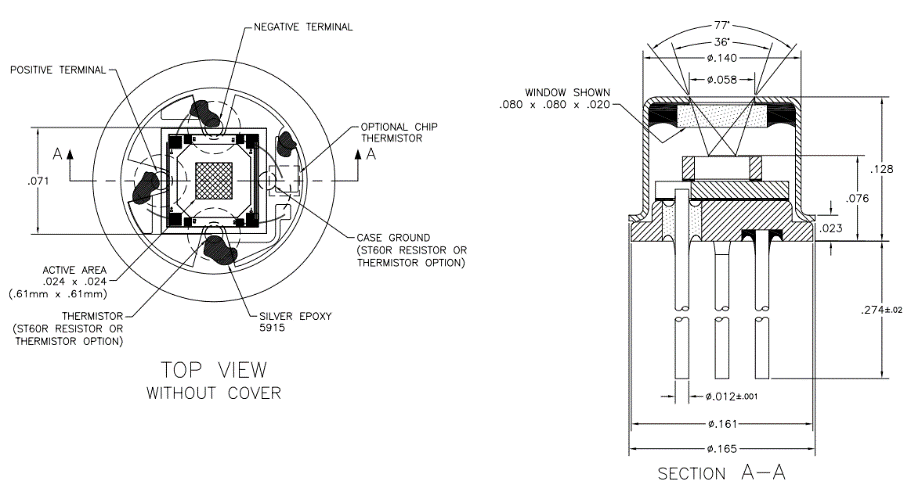
\includegraphics[scale=1]{figs/ST60Micro.png}
   \caption{ST60Micro diagram from the datasheet}
   \label{fig:ST60Micro}
\end{figure}

\subsubsection{TMP006}
The TMP006 is a fully integrated infrared sensor measuring only 1.6$\times$1.6$\times$0.8 mm, ideally suited for a narrow ear canal. Thermophile voltage and sensor temperature are made digitally available through hardware registers. These two values can be used to calculate the object temperature. Registers are accessed by a MCU though I\textsuperscript{2}C communication. Values are digitalized by a 16-bit on-chip ADC, eliminating the need for supporting analogue filters and amplifiers. The user guide of the TMP006 suggests that it be used to calculate the surface temperature of target objects with emissivity values greater than 0.7, and preferably greater than 0.9. The literature study revealed that the emissivity of the eardrum is 0.98, placing it well within the required range.

\subsubsection{Temperature measurement sensor choice}
The simple shape of the ST60 Micro makes it easy to mount, but the diameter of the package may not fit in smaller ear canals and leave little room for the other sensors. Therefore, the ST60 Micro is eliminated.

\medskip

The smaller package size and on-chip ADC justify the selection of the TMP006 for use in the Ear-Monitor. The TMP006 needs no separate analogue filter and amplifier. Furthermore, the manufacturer supplies detailed calibration documentation, allowing for more accurate and time effective calibration.

\section{Heart Rate}
The Ear-Monitor extracts heart rate from in or around the ear canal. The main criteria are sensor size, unobtrusiveness and the susceptibility of the signal to noise. The method- and sensor selection are discussed separately. 

\subsection{Heart rate measurement method}

The following five methods from literature are considered to measure heart rate.

\subsubsection{Ear ECG}

As shown by \cite{winokur2012wearable}, an electrocardiogram can be detected behind the ear. One electrode is placed behind the ear on the mastoid bone and the other on the back of the neck. A differential amplifier and ADC is used to acquire the signal. Table \ref{tab:EarECG_Eval} summarises the evaluation.

\begin{table}[H]
\caption{Ear ECG}
\label{tab:EarECG_Eval}
\renewcommand{\arraystretch}{1.3}	%Wat doen hierdie?
\centering
\begin{tabular}{|Q{5cm}|Q{8cm}|} 
 \hline

\includegraphics[scale=1]{figs/Image.png} & 
	\textbf{Advantages}
	\begin{itemize}[leftmargin=1em, noitemsep, topsep=2pt]
  	\item ECG is the standard method used by cardiologists to measure heart rate.
  	\item Other cardiac information can be extracted from ECG i.e. heart rhythm, heart damage and the state of the conductive heart tissue.
  	\item No pulse transit time delay.
  	\end{itemize}\\
  	
\hline
Sensor size: 10 mm  ${\diameter}$ electrodes	\newline				
Unobtrusiveness: Bad - electrode needed behind ear and on neck \newline	
Signal robustness: Noisy \citep{winokur2012wearable}. 		&
	
	\textbf{Disadvantages}
	\begin{itemize}[leftmargin=1em, noitemsep, topsep=2pt]
 	\item The sensor cannot be fitted entirely inside the ear canal.
	\item Two electrodes are needed.
  	\item Separate signal acquisition electronics are needed.
  	\end{itemize}\\
 
\hline
\end{tabular}
\end{table}

\subsubsection{Ear PPG}
A LED and photodiode are used to detect variation in subcutaneous tissue blood volume due to the beating heart. Literature identifies three possible locations: inside the ear canal, the earlobe and the concha. With unobtrusiveness in mind, the ear canal method is selected. This means reflective PPG is used. Table \ref{tab:EarPPG_Eval} summarises the evaluation.

\begin{table}[H]
\caption{Ear PPG}
\label{tab:EarPPG_Eval}
\renewcommand{\arraystretch}{1.3}	%Wat doen hierdie?
\centering
\begin{tabular}{|Q{5cm}|Q{8cm}|} 
 \hline

\includegraphics[scale=1]{figs/Image.png} 		& 	

	\textbf{Advantages}
	\begin{itemize}[leftmargin=1em, noitemsep, topsep=2pt]
	\item A substantial pressure pulse can be detected in and around the ear.
	\item Pulse oximetry, a type of PPG, is a tried and tested way of measuring heart rate and SpO\textsubscript{2}.
	\item Respiratory related characteristics like amplitude modulation, respiratory-induced intensity variation and frequency modulation can be found 	only in PPG signals and can be used to determine respiratory rate.
	\end{itemize}\\

\hline
Sensor size: Smallest - 1.9$\times$2.6$\times$0.8 mm	\newline		
Unobtrusiveness: Good - fits inside ear canal	\newline	
Signal noise: Low - clear pressure wave visible \citep{da2010ear}	&

	\textbf{Disadvantages}
	\begin{itemize}[leftmargin=1em, noitemsep, topsep=2pt]
 	\item PPG is susceptible to motion artefacts and variation in blood profusion.
 	\item Few PPG sensor packages are available to fit inside the ear canal.
  	\item Using separate LEDs and photo detectors increases the complexity  and size for the proof of concept Ear-Monitor.
  	\end{itemize}\\
 
 \hline
\end{tabular}
\end{table}

\subsubsection{Ear BCG}
A pressure sensitive sensor or accelerometer is placed inside the ear canal to detect the mechanical effects of the pulsating heart. Table \ref{tab:EarBCG_Eval} summarises the evaluation.

\begin{table}[H]
\caption{Ear BCG}
\label{tab:EarBCG_Eval}
\renewcommand{\arraystretch}{1.3}	%Wat doen hierdie?
\centering
\begin{tabular}{|Q{5cm}|Q{8cm}|} 
 \hline

\includegraphics[scale=1]{figs/Image.png}		& 

	\textbf{Advantages}
	\begin{itemize}[leftmargin=1em, noitemsep, topsep=2pt]	  
	\item Pressure sensors can be made small enough for the limited space in the ear canal.
	\item Accelerometer can also be used to measure respiratory rate.
	\end{itemize}\\

\hline
Sensor size: Smallest - 3$\times$3$\times$1 mm	\citep{Accelerometer}		\newline								
Unobtrusiveness: A part of the sensor protrudes from the ear, can be made smaller 	\newline	
Signal noise: High \citep{da2010ear, winokur2012wearable} 							&	
 
	\textbf{Disadvantages}
	\begin{itemize}[leftmargin=1em, noitemsep, topsep=2pt]	
	\item The signal detected by \cite{da2010ear} and \cite{winokur2012wearable} appears noisy and detecting beats are troublesome.
	\item This method is influenced by motion artefacts to such an extent that it is unusable for most forms of practical use.
 	\end{itemize}\\
 
\hline
\end{tabular}
\end{table}

\subsubsection{Phonocardiogram}
A microphone is placed inside the ear canal and identifies heart beats by analysing the sound produced by the cardiac cycle. Table \ref{tab:EarPhonocardiogram_Eval} summarises the evaluation.

\begin{table}[H]
\caption{Ear Phonocardiogram}
\label{tab:EarPhonocardiogram_Eval}
\renewcommand{\arraystretch}{1.3}
\centering
\begin{tabular}{|Q{5cm}|Q{8cm}|} 
\hline

\includegraphics[scale=0.8]{figs/Image.png} 		& 	

	\textbf{Advantages}
	\begin{itemize}[leftmargin=1em, noitemsep, topsep=2pt]	  
	\item Can be used to detect breathing as well, as shown by \cite{goverdovsky2016hearables}.
	\end{itemize}\\
	
\hline
Sensor size: 3.35$\times$2.5$\times$ \SI{0.98}{\milli\meter} \citep{Microphone}	\newline	
Unobtrusiveness: Can fit inside the ear canal  \newline	
Signal noise: High 	&
 
	\textbf{Disadvantages}
	\begin{itemize}[leftmargin=1em, noitemsep, topsep=2pt]
	\item Sounds from other sources like movement and speaking can corrupt the signal.
	\end{itemize}\\
 
 \hline
\end{tabular}
\end{table}

\subsubsection{Heart rate method choice}
Ear PPG is selected as the Ear-Monitor's method of measuring heart rate. PPG produces a clear signal that will allow for accurate beat detection. This method can also be incorporated into the SpO\textsubscript{2} measurement sensor, eliminating the need for two different sensors. The entire sensor fit inside the ear canal, making it unobtrusive. This method is also less susceptible to noise than ear BCG or a phonocardiogram.

\subsection{Heart rate measurement sensor}
Reflexive ear canal PPG is selected to measure heart rate. Three PPG sensors options are considered namely: separate LEDs and photodetector, the NJL5501R from JRC and the MAX30100 by Maxim Integrated.

\subsubsection{Separate LEDs and photodetector}
SMD LEDs are used with one or more photo detectors. The components are mounted on a thin PCB and placed in the ear probe. The LEDs and photo detectors can be placed in various precise configurations and a wider choice of individual transducers can be used. Additional analogue electronics are needed to drive the LEDs, conditioning the detector signal output and compensate for ambient lighting. A commercial integrated analogue front-end chip like Texas Instruments' AFE4400 is used to perform this task.

\subsubsection{NJL5501R}
The NJL5501R is a surface mounted photo-emitter and -detector contained in one 1.9$\times$2.6$\times$0.8 mm package shown in Figure \ref{fig:NJL5501R}. Red and infrared LEDs make it suitable for reflective pulse oximetry and heart beat detection. Its small size allows it to fit in the ear canal while leaving adequate space for other sensors. It requires all the same supporting electronics such as using the separate LEDs and a photo-detector method.

 \begin{figure}[h]
   \centering
   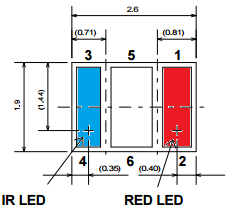
\includegraphics[scale=1]{figs/NJL5501R.png}
   \caption{NJL5501R diagram from the datasheet}
   \label{fig:NJL5501R}
\end{figure}

\subsubsection{MAX30100} 
The MAX30100 is a single chip pulse oximeter and heart rate detector. It has red and infrared LEDs, a photodetector, a 16-bit ADC and digital filters all in one 5.6$\times$2.8$\times$1.2 mm, 14-Pin package. The LEDs and photodetector are in the same plane, which means it operates in reflective mode. Like the TMP006 it uses the I2C protocol to communicate with a MCU. Configuration registers allow the designer to specify sample rate, LED currents and LED pulse width. Figure \ref{fig:MAX30100_Diagram} shows a block diagram of the internal systems of the MAX30100.

\begin{figure}[H]
   \centering
   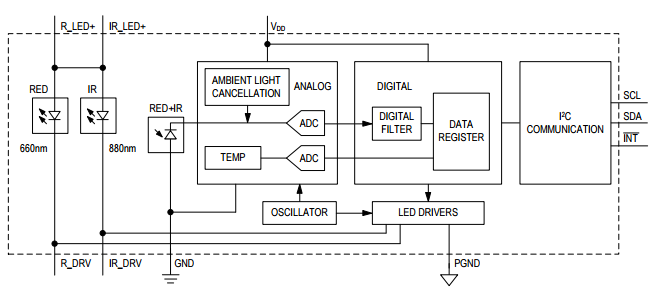
\includegraphics[scale=1]{figs/MAX30100_Diagram.png}
   \caption{MAX30100 block diagram from the datasheet}
   \label{fig:MAX30100_Diagram}
\end{figure}

The MAX30100 uses a 3.3V supply and programmable current sources to drive the LEDs, whilst digital operations are done at 1.8V. It draws between 6 and \SI{12}{\milli\ampere} mA while recording red and infrared PPGs. It has a digital 50Hz/60Hz notch filter to reject powerline interference. LEDs can be varied individually from 0 to \SI{50}{\milli\ampere} and the alternating LED pulse widths can be varied from 0.2 to \SI{1.6}{\milli\second}. A sample rate can be selected between 5 and 1000 samples per second. An important feature of the MAX30100 is its 64-byte deep FIFO register which is used to store the output values. Each output set consists of a 16-bit red and 16-bit infrared value, which means that there are 4 bytes per output and therefore 16 sets of output values can be held in the FIFO at any time. The MCU reads 4 bytes at a time from the FIFO to obtain the latest red and infrared values.

\subsubsection{Heart rate sensor choice}
The MAX30100 is selected for use in the Ear-Monitor. It has optimized optics to guide outgoing and incoming light. It has integrated ambient light cancellation. Its entire AFE is integrated which means that no additional electronics are needed, apart from the I2C lines and power regulators. This gives it a big advantage over the more complex separate LEDs and photodetector method. Its small size and reflective mode of operation allows it to be placed inside the ear canal. Data recorded by the MAX30100 is used to calculate heart rate and SpO\textsubscript{2}. 

%Talk about the selection of the MAX30100's location on the probe

\section{Respiratory Rate}
The Ear-Monitor measures respiratory rate from inside the ear canal. The main criteria are sensor size and susceptibility to noise corruption.

\subsection{Respiratory rate measuring method}
The following three respiratory rate measuring methods from literature are considered.

\subsubsection{Accelerometer}
A small MEMS accelerometer is placed inside the ear canal and measures the movement of the head caused by breathing. Table \ref{tab:EarAccelerometer_Eval} summarises the evaluation.

\begin{table}[H]
\caption{Ear Accelerometer}
\label{tab:EarAccelerometer_Eval}
\renewcommand{\arraystretch}{1.3}
\centering
\begin{tabular}{|Q{5cm}|Q{8cm}|} 
 \hline
 

\includegraphics[scale=0.8]{figs/Image.png} 		& 	

	\textbf{Advantages}
	\begin{itemize}[leftmargin=1em, noitemsep, topsep=2pt]	  
	\item The accelerometer can serve the dual purpose of measuring breathing and heart rate, thus saving space.
	\end{itemize}\\ 
	
\hline
Sensor size: 3$\times$3$\times$\SI{1}{\milli\meter}	\citep{Accelerometer}	\newline
Noise: Very high							&	

	\textbf{Disadvantages}
	\begin{itemize}[leftmargin=1em, noitemsep, topsep=2pt]	  
	\item This method is extremely vulnerable to noise form other movements.
	\end{itemize}\\ 

 \hline
\end{tabular}
\end{table}

\subsubsection{Microphone}
A microphone is placed inside the ear canal and records the sound of air moving through the respiratory tracts, allowing the respiratory rate to be determined. Table \ref{tab:EarMicrophone_Eval} summarises the evaluation.

\begin{table}[H]
\caption{Ear Microphone}
\label{tab:EarMicrophone_Eval}
\renewcommand{\arraystretch}{1.3}	%Wat doen hierdie?
\centering
\begin{tabular}{|Q{5cm}|Q{8cm}|} 
 \hline
 
\includegraphics[scale=0.8]{figs/Image.png} 		& 	
 
	\textbf{Advantages}
	\begin{itemize}[leftmargin=1em, noitemsep, topsep=2pt]	  
	\item The microphone can serve the dual purpose of measuring breathing and heart rate, thus saving space.
	\end{itemize}\\ 

\hline
Sensor size: 4$\times$3$\times$\SI{1}{\milli\meter} \citep{Microphone}		\newline
Noise: Very high	&

	\textbf{Disadvantages}
	\begin{itemize}[leftmargin=1em, noitemsep, topsep=2pt]	  
	\item This method is extremely vulnerable to noise form other sounds, like talking or ambient noise.
	\end{itemize}\\ 
	
 \hline
\end{tabular}
\end{table}

\subsubsection{Respiratory related heart rate characteristics}
The variations in heart rate are used to determine the respiratory rate. These include amplitude modulation, respiratory-induced intensity variation and frequency modulation of the heart rate in synchronization with the respiration rate. Table \ref{tab:EarRRHRC_Eval} summarises the evaluation.

\begin{table}[H]
\caption{Respiratory related heart rate characteristics}
\label{tab:EarRRHRC_Eval}
\renewcommand{\arraystretch}{1.3}	%Wat doen hierdie?
\centering
\begin{tabular}{|Q{5cm}|Q{8cm}|} 
 \hline
 
\includegraphics[scale=0.8]{figs/Image.png} &
  			
  	\textbf{Advantages}
	\begin{itemize}[leftmargin=1em, noitemsep, topsep=2pt]	  
	\item No dedicated sensor is needed.
	\item Less susceptible to noise than the accelerometer or microphone method.
	\end{itemize}\\ 
	
\hline
Sensor size: No sensor needed	\newline
Noise susceptibility: Low			&	

	\textbf{Disadvantages}
	\begin{itemize}[leftmargin=1em, noitemsep, topsep=2pt]	  
	\item Only steady and relatively slow respiratory rates can be detected.
	\end{itemize}\\
	
\hline
\end{tabular}
\end{table}

\subsubsection{Respiratory Rate Sensor Choice}
Respiration measurement through analysing respiratory related heart rate characteristics, of which heart rate frequency modulation through respiratory sinus arrhythmia (RSA) is found to be the most detectable, is selected for use in the Ear-Monitor. This method saves space by not requiring a dedicated sensor. It is also the least susceptible to noise from other sources. No sensor selection is needed for this vital sign, as all the work is done by the micro controller.

\section{Blood oxygen saturation}
Pulse oximetry is the only practical way for the Ear-Monitor to measure blood oxygen saturation. The MAX30100 selected for measuring heart rate is equipped for this task. A red and infrared LED as well as a photo-detector are available for the joint function for measuring heart rate and SpO\textsubscript{2}.

\section{Final concept}
The final concept is obtained by combining the methods and sensors selected in this chapter which are summarised as follows:

\begin{itemize}
\item Core body temperature is measured by the TMP006 infrared sensor, located at the tip of the Ear-Monitor's ear probe and pointed at the tympanic membrane.
\item Heart rate is measured by the MAX30100 reflective pulse oximeter placed on the side of the ear probe and facing the canal wall. The PPG signal is used to calculate heart rate.
\item Respiratory rate is calculated by analysing respiratory sinus arrhythmia (RSA), which is the frequency modulating respiratory related heart rate characteristic.
\item SpO\textsubscript{2} is also measured by the MAX30100. The red and infrared PPGs obtained from the ear canal wall are used for this calculation.
\end{itemize}

\medskip

Additionally, a microcontroller unit (MCU), battery and wireless transceiver are selected for the Ear-Monitor. The Arduino Pro Mini MCU has the necessary I/O pins for serial communication with the sensors and wireless module. It is also easy to program, making it ideal for the proof of concept version of the Ear-Monitor. Lithium polymer (LiPo) batteries are currently the best choice when regarding capacity, compactness, rechargeability and price. It is therefore selected to supply the power to the Ear-Monitor. Bluetooth is the typically used standard for transmitting data over short distances and is supported by most modern smart devices. The HC-05 Bluetooth modem is selected and allows the Ear-Monitor to send data to a supporting device through a wireless connection. Figure \ref{fig:EarMonitor_Concept} shows a diagram of the Ear-Monitor concept with a more detailed drawing of the ear probe with the selected sensors.

\begin{figure}[H]
\centering
\graphicspath{{figs/}}
\input{figs/EarMonitor_Concept.pdf_tex}
\caption{Ear-Monitor concept with components labelled}
\label{fig:EarMonitor_Concept}
\end{figure}

